\documentclass{article}

\usepackage{fullpage}
\usepackage{amsmath}
\usepackage{graphicx}
\usepackage[utf8]{inputenc}
\usepackage{pdfpages}
\usepackage{graphicx}
\usepackage{multicol}
\usepackage{tikz}
\usepackage{pgfplots}
\pgfplotsset{compat=1.12}


\title{Examen final de Cálculo Diferencial}
\author{M. en C. Reinaldo Arturo Zapata Peña}

\begin{document}
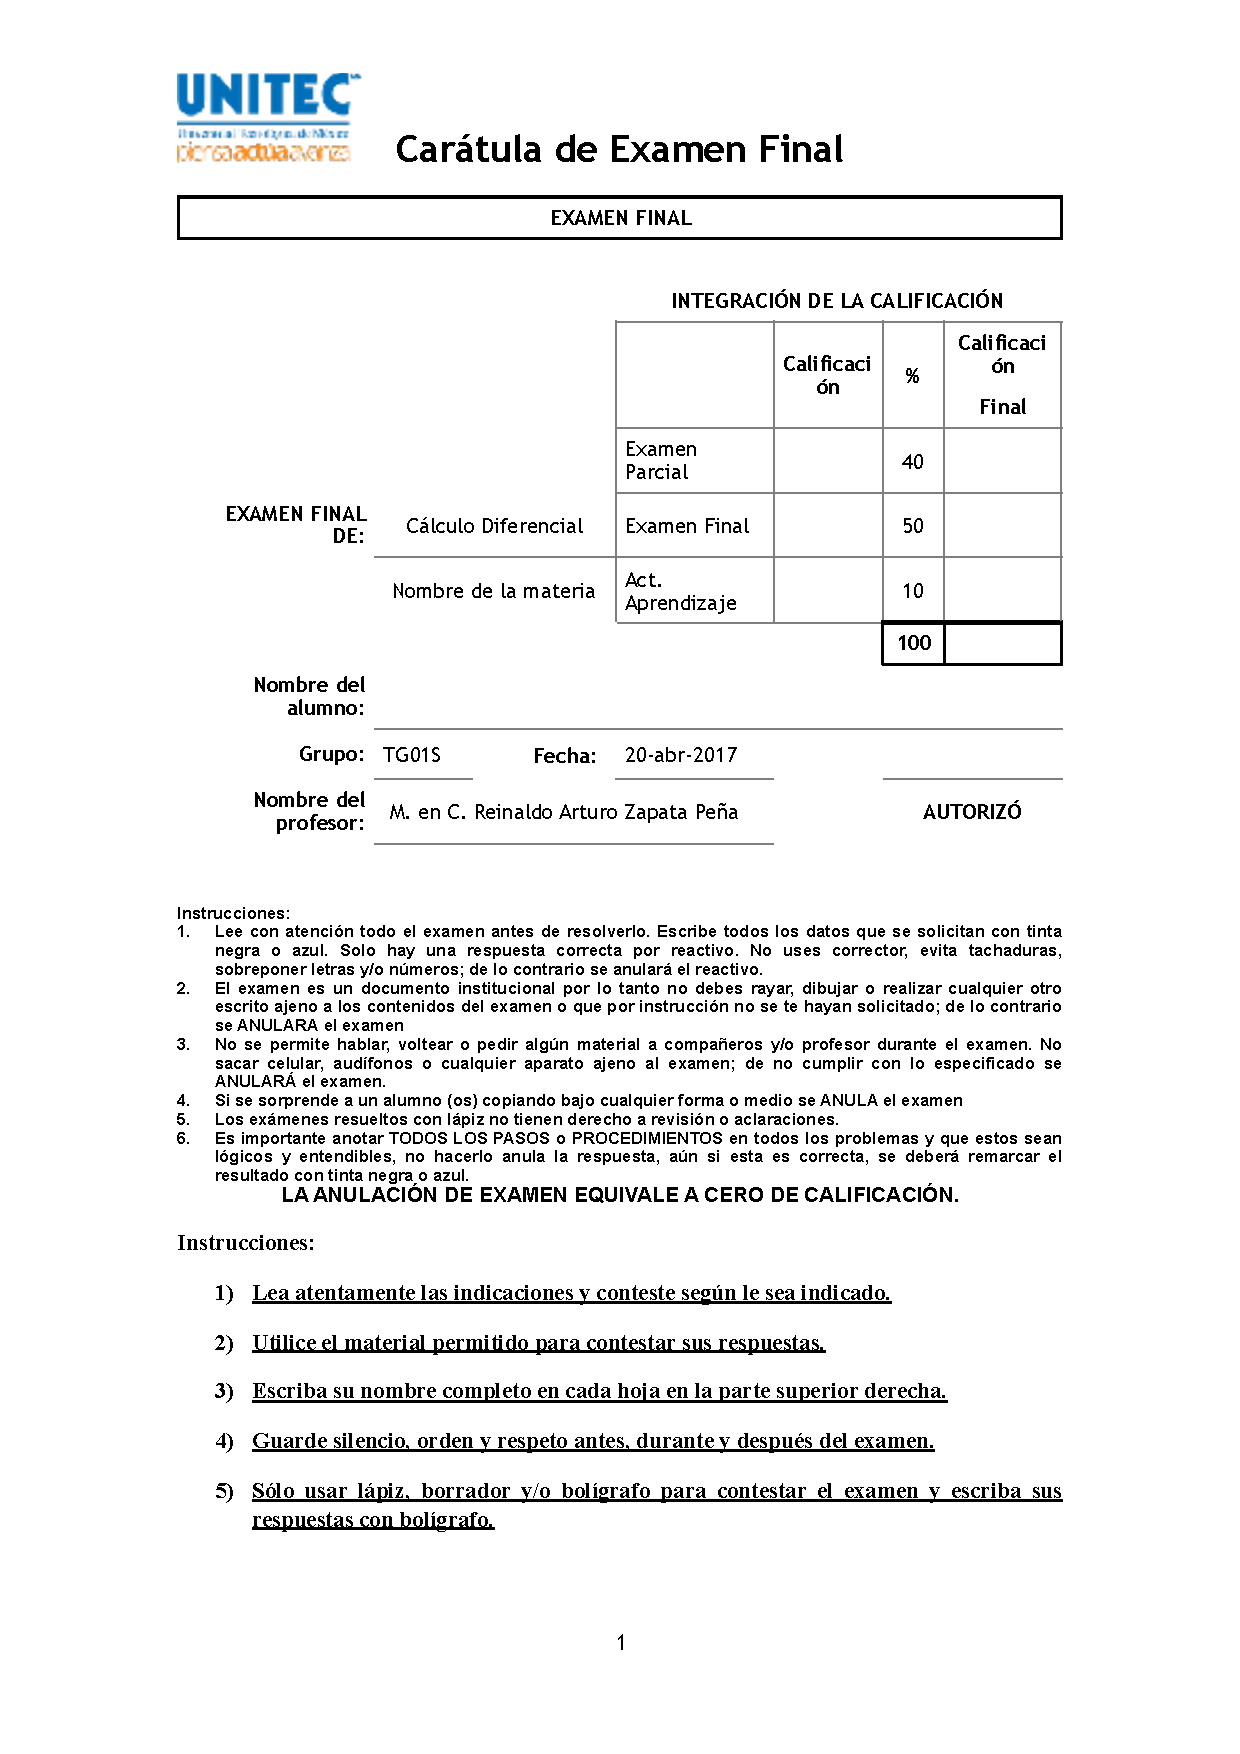
\includepdf[pages=-]{car-final-calc}

\section{Teoría} % (fold)
\label{sec:teoria}


\begin{figure}[b]
    \centering
  \begin{tikzpicture}
    \begin{axis}[
     x=60, y=30, clip=false, xmin=-0.30,xmax=2.2*pi, xlabel= $x$,
     ylabel=$f(x)$, ymin=-2.2,ymax=2.7, axis lines=middle,
     xtick={0,1.57,3.14,4.71,6.28}, xticklabel style = {fill=white},
     xticklabels={$0$, $\displaystyle\frac{\pi}{2}$,
     $\displaystyle\pi\,$,$\,\,\,\displaystyle\frac{3\pi}{2}$,$\,2\pi$}, set
     layers = axis on top ]
     \draw (axis cs:0,1) -- (axis cs:6.28,1);
     \draw (axis cs:0,2) -- (axis cs:6.28,2);
     \draw (axis cs:0,-1) -- (axis cs:6.28,-1);
     \draw (axis cs:0,-2) -- (axis cs:6.28,-2);
     \draw (axis cs:1.57,2) -- (axis cs:1.57,-2);
     \draw (axis cs:3.14,2) -- (axis cs:3.14,-2);
     \draw (axis cs:4.71,2) -- (axis cs:4.71,-2);
     \draw (axis cs:6.28,2) -- (axis cs:6.28,-2);
     \draw (axis cs:0.78,2) -- (axis cs:0.78,-2);
     \draw (axis cs:2.36,2) -- (axis cs:2.36,-2);
     \draw (axis cs:3.93,2) -- (axis cs:3.93,-2);
     \draw (axis cs:5.50,2) -- (axis cs:5.50,-2);
    \end{axis}
  \end{tikzpicture}
    \caption{especio  para graficar funciones.}
    \label{fig:graficar}
\end{figure}
\begin{enumerate}
\item Explique qué es una función par e impar.
\hfill \textbf{6 puntos.}

\item Haciendo uso de la figura \ref{fig:graficar}, haga un bosquejo de las
funciones $f(x)=\cos(2x)$ y $g(x)=2\sin(x)$ para el intervalo $0 \leq x \leq
2\pi$. Identifica cada una de ellas etiquet\'andolas.
\hfill \textbf{6 puntos.}

\item Explique con sus palabras que interpretación geométrica tiene la
derivada de una función.
\hfill \textbf{6 puntos.}

\item Si para una recta tangencial a una función $f(x)$ se conoce el punto
($a$,$f(a)$) y la pendiente de la recta tangente $m_{\text{tan}}$, escriba el
procedimiento para encontrar la recta perpendicular a la función en dicho punto.
\hfill \textbf{6 puntos.}

\item Explique con sus palabras que establece el teorema de l'H\^opital y las
situaciones en las que se puede utilizar.
\hfill \textbf{6 puntos.}

\end{enumerate}

% section teoría (end)



\section{Problemas} % (fold)
\label{sec:problemas}

\begin{enumerate}

\item Sea la función $f(x)= 2x^{2} -3x + 8$ encuentre las rectas tangente y
perpendicular a dicha función en el punto $x=4$. Indique además cual es el
ángulo que forma dicha recta respecto al eje positivo de las $x$.

\hfill \textbf{9 puntos.}

\item Dadas las siguientes funcines, 
\hfill \textbf{9 puntos.}

\begin{align}
f(x) &= \frac{x^{2} - 4x  + 4 }{x+5}, \label{eq:lim1}
\\
g(x) &= \frac{\sin^{2}(x)}{x^{2}-25}, \label{eq:lim2}
\end{align}
encuentre los puntos para los cuales estas funciones son indeterminadas.

\item Utilizando las funciones del inciso anterior, determine el límite para la
Ec. \eqref{eq:lim1} cuando $x\rightarrow3$ y el límite para la Ec.
\eqref{eq:lim2} cuando $x\rightarrow2$.
\hfill \textbf{9 puntos.}

\item Utilizando nuevamente las Ecs. \eqref{eq:lim1} y \eqref{eq:lim2} y la
regla de l'H\^opital, determine el límite de cada una de las funciones cuando
$x\rightarrow-5$.
\hfill \textbf{9 puntos.}

\newpage
\item Usando la regla de la caden y las reglas de derivación encuentre la
derivada de las siguientes funciones.

\hfill \textbf{9 puntos.}

\noindent
\begin{minipage}{0.5\linewidth}
\begin{align}
\label{eq:f(x)} f(x) &= \tan(x)  \\
\label{eq:g(x)} g(x) &= \ln(x^{2})e^{2x^{3}}  \\
\label{eq:h(x)} h(x) &= \frac{\sin(2x)}{e^{x^{2}}}  
\end{align}
\end{minipage}%
\begin{minipage}{0.5\linewidth}
\begin{align}
\label{eq:i(x)} i(x) &= 3x^5\cos(2x)\sin(5x^{3})  \\
\label{eq:j(x)} j(x) &= \sin^{3}(2x^{2})  \\
\label{eq:k(x)} k(x) &= \frac{1}{e^{2x^{5}}}  
\end{align}
\end{minipage}

\item Si la posición de un sistema en movimiento está dada por la función
\hfill \textbf{8 puntos.}
\begin{equation}\label{eq:poscion}
x(t)= 5t^{2} - 6t + 8
\end{equation}
determine la velocidad y la aceleración de la partícula en función del tiempo.

\item Usando la Ec. \eqref{eq:poscion} determine el valor mínimo para la
posición de la partícula.
\hfill \textbf{8 puntos.}

\item Encuentre la tercera y cuarta derivada de la Ec. \eqref{eq:k(x)}.
\hfill \textbf{9 puntos.}

\clearpage

\section{Respuesas} % (fold)
\label{sec:respuesas}

% section respuesas (end)

\end{enumerate}

\clearpage

\section{Respuestas} % (fold)
\label{sec:respuestas}

% section respuestas (end)






% section problemas (end)

\end{document}

y(x)= 5*x^2 - 6*x + 8




